\section[\textbf{TPM of Matter} \& \EnergyInteractionModel{}]{Practicing the \ThreePhaseModel{}; Introducing the \EnergyInteractionModel{}}
\label{act1.1.3}

\note{Timing: \unit[40]{min}}{

	\subsubsection*{Purpose}
		\begin{itemize}
			\item Provide practice applying both the \ThreePhaseModel{} and the \EnergyInteractionModel{} to various phenomena.
		\end{itemize}

	\subsubsection*{Learning Outcomes}
		\begin{itemize}
			\item Capable of drawing \EnergyDiagrams{} for simple physical processes
		\end{itemize}
}

\begin{overview}
	\noindent
	{\bfseries Overview:} We briefly interrupt our efforts of making sense of the heat pack to get a bit of practice using the \ThreePhaseModel{} and to introduce the \EnergyDiagram{}.
\end{overview}

\note{}{``All members of your group must now go to the board and work on the following together.'' You must enforce this. Students need to interact with each other and not let one or two students do all the work.  Having them all at the board really helps here.}

\noindent\textbf{Your instructor will assign one or more of the following physical processes to your small group:}

\begin{enumerate}[(a)]
	\item Cooling a piece of solid copper (Cu) from \unit[500]{\textdegree C} to \unit[350]{\textdegree C}.
	\item Warming a piece of ice from \unit[-20]{\textdegree C} to the melting point.
    	\item Condensing steam completely to liquid at \unit[100]{\textdegree C}.
	\item Completely sublimating a chunk of dry ice at \unit[-79]{\textdegree C}.
	\item Partially melting 25\% of ice initially at \unit[0]{\textdegree C}.
	\item Heating a piece of copper initially at \unit[300]{\textdegree C} until it is half melted.
	\item Cooling and completely freezing \ce{H2O} initially at \unit[80]{\textdegree C}.
\end{enumerate}

\noindent {\bfseries For each of these processes, sketch the following on your whiteboard and be prepared to explain to the whole class:}

\begin{enumerate}[(i)]
	\item A complete \TempGraph{} (remember, this is the graphical part of the \ThreePhaseModel{}) with the initial and final states clearly marked; 
	
	{\bfseries and }
	
	\item An {\em open} \EnergyDiagram{}. Refer to ``Steps Involved in Using the \EnergyDiagram'' on the \EnergyInteractionModel{} summary on your table. Try your hand at translating your \EnergyDiagram{} into an algebraic expression of energy conservation.
\end{enumerate}

	
\begin{center}
%	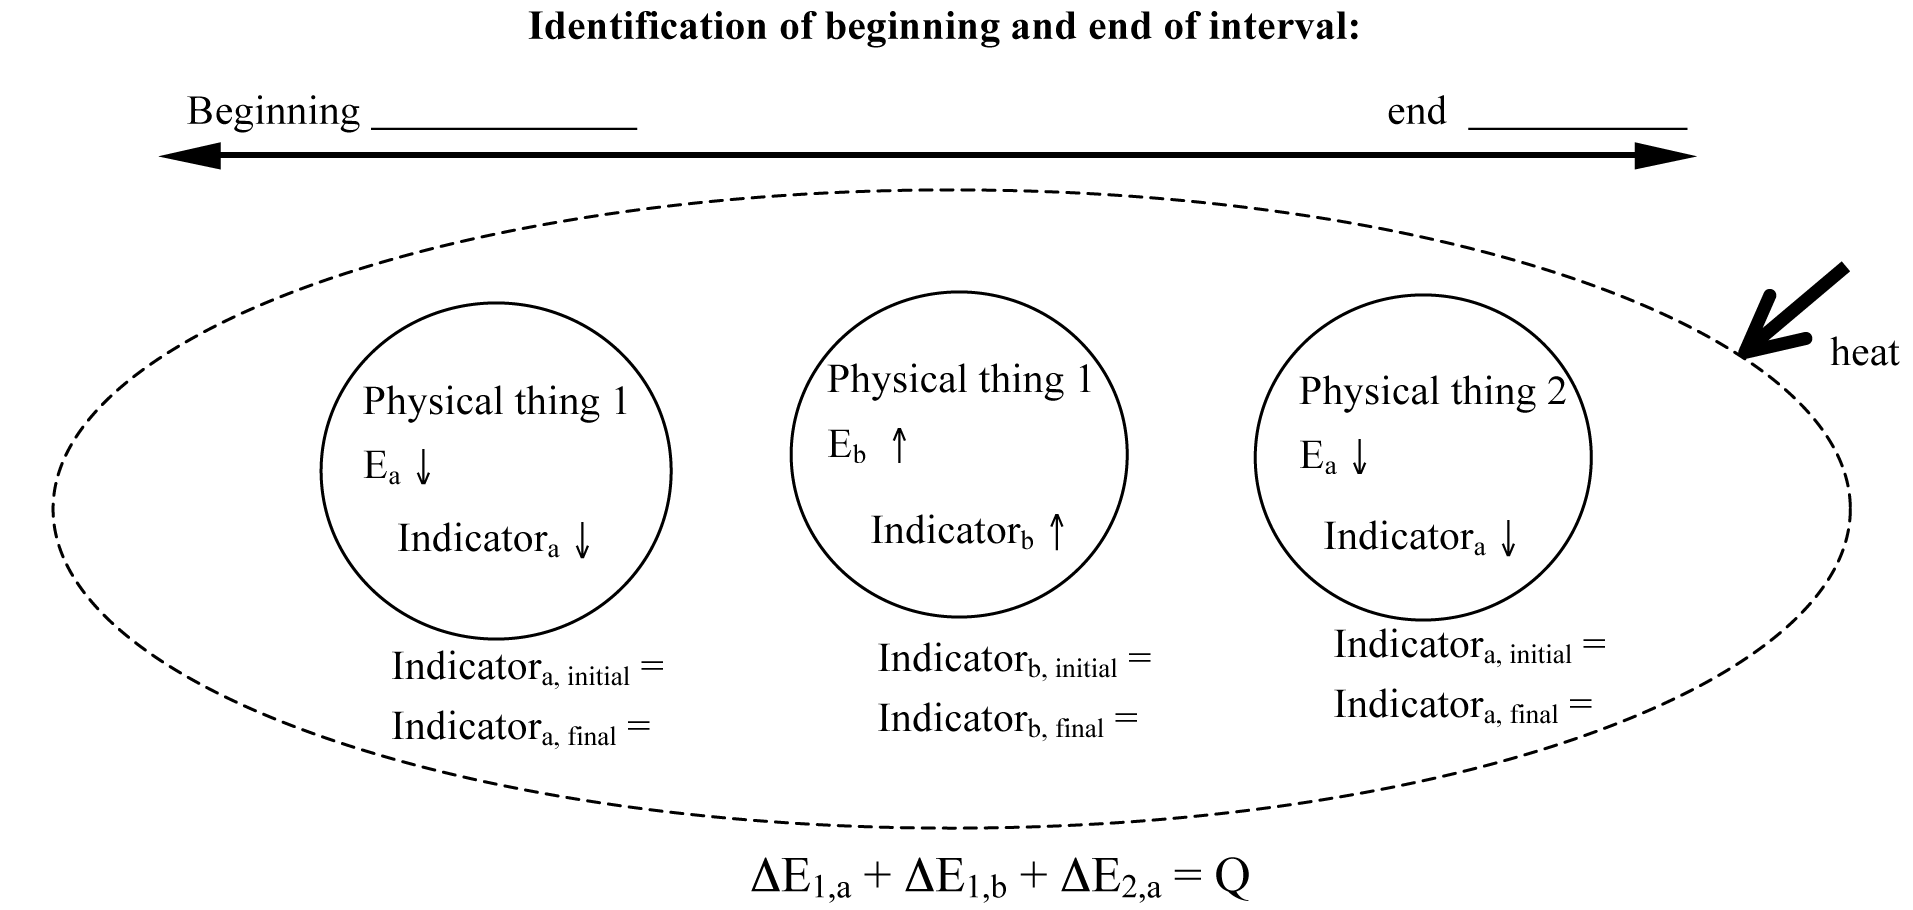
\includegraphics[width=0.7\linewidth]{E-ID}
	
\begin{tikzpicture}[thick,scale=0.75, every node/.style={transform shape}]
    % draw horizontal line   
    \draw[-{Stealth[scale=1.2]}, line width=1pt] (0,0) -- (10.2,0);

    % draw vertical lines
    \foreach \x in {0.5,9.5}
      \draw[line width=1pt] (\x cm,3pt) -- (\x cm,-3pt);

    % title the diagram
    \draw (5,0) node[above=18pt] {\scriptsize{\textbf{Identification of \emph{beginning} and \emph{end} of interval:}}};

    % draw nodes along the interval timeline
    \draw (0.5,0) node[below=3pt] {\scriptsize{initial conditions}} node[above=3pt] {\emph{beginning}};
    \draw (9.5,0) node[below=3pt] {\scriptsize{final conditions}} node[above=3pt] {\emph{end}};

    % draw the physical system boundary
    \draw [dashed,orange,line width=1pt] (5,-2.75) ellipse (6cm and 2.25cm) node[above=1.5cm] {\textbf{\emph{physical system}}};
    
    % draw energy systems
    \draw (2,-3) node[draw,circle,blue,minimum size=2.25cm,inner sep=0pt,align=center]  {\color{darkgray}\tiny{indicator $a$}\\[.5ex]$\downarrow E_\text{1,a}$\\\color{darkgray}\tiny{$a_i =$}\\[-1.2ex]\color{darkgray}\tiny{$a_f =$}} node[orange,above=1.1cm] {\scriptsize{physical thing 1}};
    \draw (5,-3.25) node[draw,circle,blue,minimum size=2.25cm,inner sep=0pt,align=center]  {\color{darkgray}\tiny{indicator $b$}\\[.5ex]$\uparrow E_\text{1,b}$\\\color{darkgray}\tiny{$b_i =$}\\[-1.2ex]\color{darkgray}\tiny{$a_f =$}} node[orange,above=1.1cm] {\scriptsize{physical thing 1}};
    \draw (8,-3) node[draw,circle,blue,minimum size=2.25cm,inner sep=0pt,align=center]  {\color{darkgray}\tiny{indicator $a$}\\[.5ex]$\downarrow E_\text{2,a}$\\\color{darkgray}\tiny{$a_i =$}\\[-1.2ex]\color{darkgray}\tiny{$a_f =$}} node[orange,above=1.1cm] {\scriptsize{physical thing 2}};    

    % draw heat arrow
    \draw[{Stealth[scale=1.2]}-, line width=1pt, blue] (10,-2.25) -- (11,-1.5)  node[right=0cm] {heat Q};
    
    % write energy conservation equation
    \draw (5,-6) node[] {$\Delta E_\text{1,a} + \Delta E_\text{1,b} + \Delta E_\text{2,a} = Q$};
    \draw (3,-6) node[above=6pt] {\scriptsize{$(-)$}};
    \draw (4.6,-6) node[above=6pt] {\scriptsize{$(+)$}};
    \draw (6.15,-6) node[above=6pt] {\scriptsize{$(-)$}};
    \draw (7.35,-6) node[above=6pt] {\scriptsize{$(+)$}};

\end{tikzpicture}
\end{center}

\note{Procedure}{
	\begin{itemize}
		\item Assign one process to each \SG{}.  If a \SG{} finishes early, have them do another.  You could also have them tell you how to draw one on the board.
		\item Tell students to study the example of an \EnergyDiagram{} on two-page blue model summary.
		\item Remind the students that all of these are very straightforward, and should be mastered quickly.  Any complicated process will require the coordination of multiple energy systems. These should be thought of as ``exercises.''
	\end{itemize}
	
	You do not necessarily have to get through all of these by the end of DL, but if you can at least cover the first three they should be able to finish the remainder. They are also assigned as part of the \FNTs.
	
	Some of the processes are not stipulated sufficiently to guarantee a unique diagram (e.g., Process~3). That's ok. They can discuss/compare the different possibilities.
}


\noindent \textbf{Again, \emph{you need to be prepared} to explain and describe the process you have been assigned to the whole class using both models.} When you use the \ThreePhaseModel{} trace the process with your finger as you describe it. Make sure you clearly show the beginning and ending points of the process in the diagram.\\

\textbf{NOTE:} You will have an opportunity to rework these examples in the \hyperref[\FNT1.1.3-1]{homework}. These are all very straightforward once you're familiar with the basic ideas of the two models. Working through these examples will also give you practice in applying the models and using the representations with a variety of phenomena. It is very important that you can do this quickly and correctly (i.e., it should become \emph{second nature} to you). When applying these models to make sense of more complicated phenomena, e.g., on a quiz, it is crucial that you are not stumbling over the basics.

%\todo[inline]{This WCD seems squished to the Note above it. I have no idea why this happens and how to fix it. It'd be good if this could be formatted consistently throughout the book. Maybe using an environment?}
\WCD

\note{}{
	Have each group explain how their \TempGraph{} matches their \EnergyDiagram{}.
	
	{\em You should have already corrected any gross errors as they are putting them up.}
	
	After a group has presented, you should ask the whole class if there is anything that is left out or that should be worded in a better way, etc.  This is an opportunity to help all students see what properly drawn diagrams should be like.
	
	{\em You should have groups correct any mistakes or omissions on their diagram on the board. This helps provide closure for everyone.}
}

\note{}{
	Shown below are examples of \EnergyDiagrams{} for Processes 1 and 3.  Notice that the indicator for bond energy systems is treated differently in the diagram than indicators for other energy systems, i.e., they are not required to record specific initial and final values of mass.
	
	\begin{multicols}{2}
		Process 1\\		
		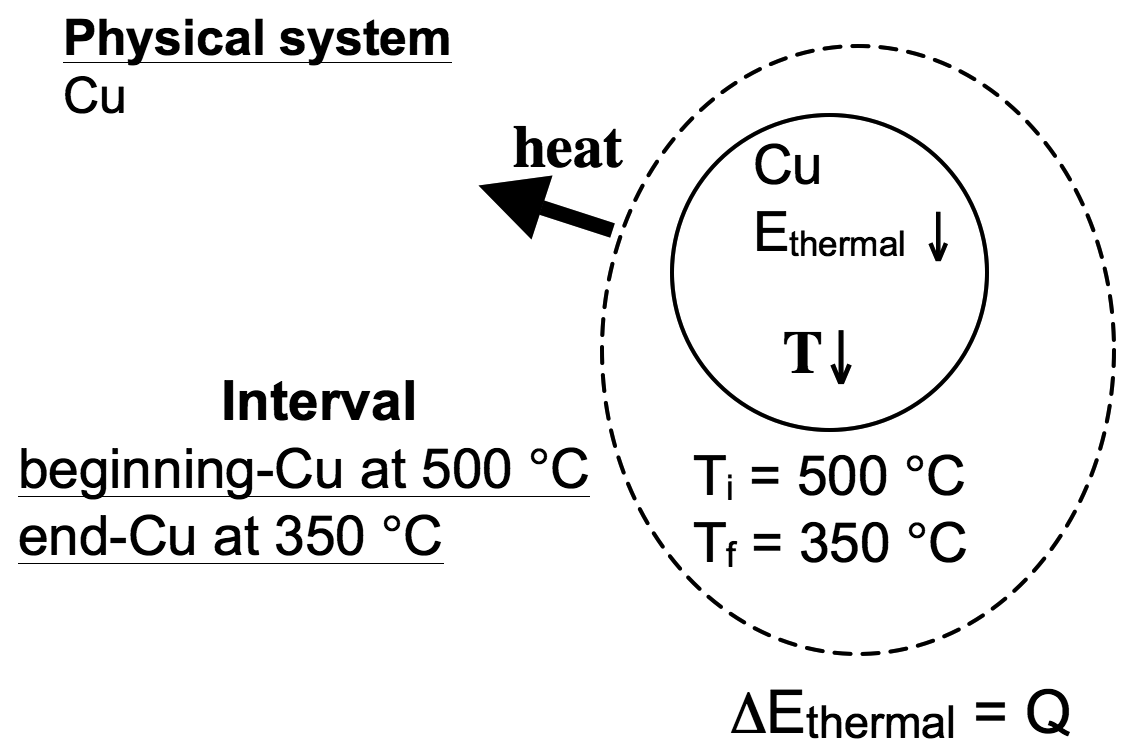
\includegraphics[width=0.9\linewidth]{act113-1}
		
		\columnbreak
		Process 3\\		
		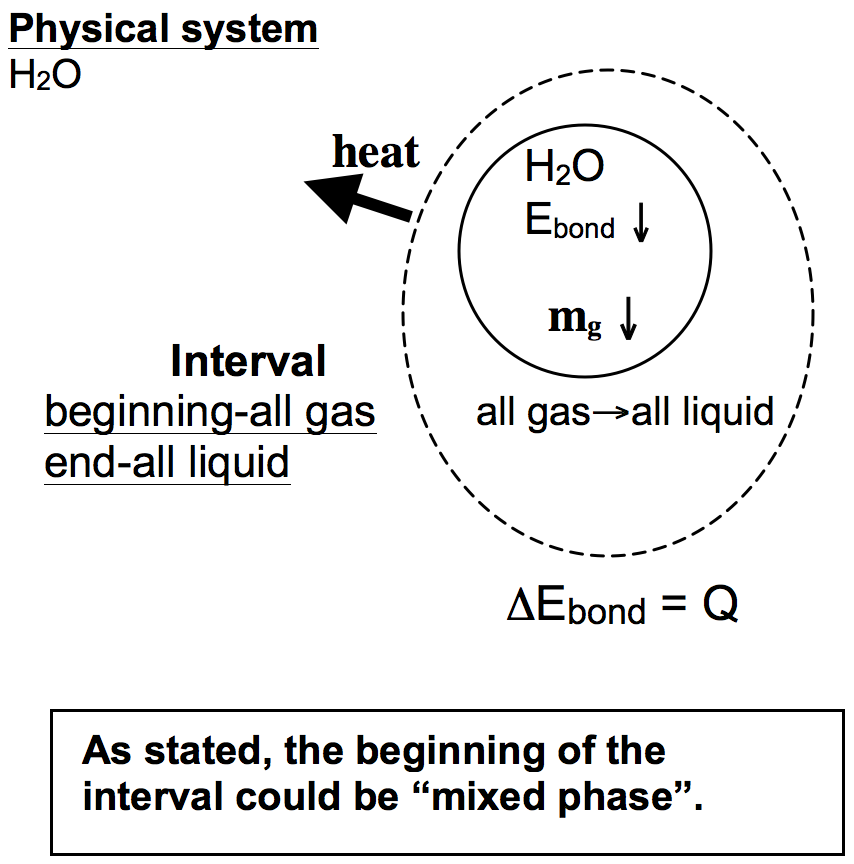
\includegraphics[width=0.9\linewidth]{act113-3}
	\end{multicols}
}